%! alt Triangle ABC with BC = 102 along the bottom, CA = 136 and AB = 153, and the point P inside it joined to the three vertices, with PA = 96, PB = 81 and PC = 48. The three equal angles PAB, PBC and PCA are marked omega. Triangle PAB is shaded; its angle at P is 180 degrees minus angle B.
%! after_paragraph 1
%! scale 1/20
%! let S = 868952484
% The shared preamble of every Cevian figure. pipeline/figures turns these colours into theme-aware paint,
% and refuses any other colour, so draw only with them:
%   figink (lines and labels), figaux (construction lines), figaccent (the object the argument turns on),
%   figtint and figaccenttint (light fills).
\documentclass[border=1.5pt]{standalone}
\usepackage{tkz-euclide}
\definecolor{figink}{RGB}{0,0,0}
\definecolor{figaux}{RGB}{85,85,85}
\definecolor{figaccent}{RGB}{192,57,43}
\definecolor{figtint}{RGB}{221,221,221}
\definecolor{figaccenttint}{RGB}{245,213,208}
% tkz-euclide's defaults draw circles, compasses and marks in 50% grey and fill points with a tint.
\makeatletter
\def\tkz@otherlinecolor{figink}
\def\tkz@euc@circlecolor{figink}
\def\tkz@euc@compasscolor{figink}
\def\tkz@euc@mkcolor{figink}
\def\tkz@mk@fill{figink}
\def\tkz@euc@pointfillcolor{figink}
\makeatother
\tkzSetUpLine[color=figink,line width=.7pt]
\tkzSetUpArc[color=figink,line width=.7pt]
\tkzSetUpCompass[color=figink,line width=.5pt]
\tkzSetUpPoint[color=figink,fill=figink,size=3.1pt]
\tikzset{
  every picture/.style={line cap=round,line join=round,color=figink},
  circle style/.append style={color=figink,line width=.7pt},
  aux/.style={color=figaux,line width=.45pt,dash pattern=on 2.6pt off 2pt},
  key/.style={color=figaccent,line width=1pt},
  mk/.style={color=figink,line width=.5pt},
  lbl/.style={color=figink,inner sep=2.2pt},
  len/.style={color=figink,inner sep=1.5pt,font=\small},
}

\begin{document}
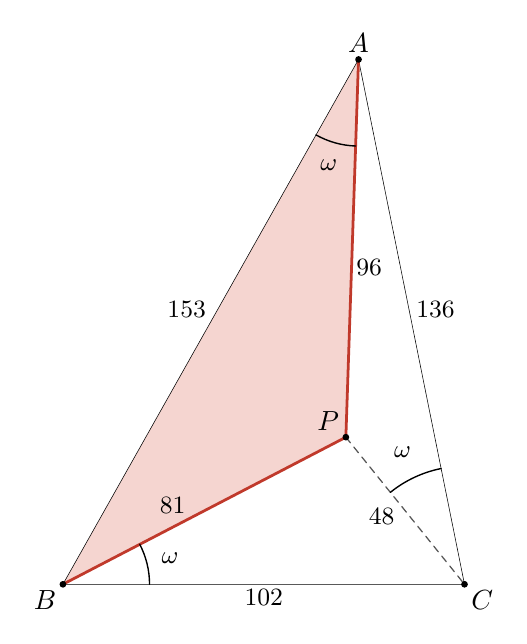
\begin{tikzpicture}
\tkzDefPoint(0.0,0.0){B} %! B = (0, 0)
\tkzDefPoint(5.1000000,0.0){C} %! C = (102, 0)
\tkzDefPoint(3.7541667,6.6654882){A} %! A = (15317/204, sqrt(23409 - (15317/204)**2))
\tkzDefPoint(3.5933824,1.8681818){P} %! P = ((243547236*x(A) + 432972864*102)/S, 243547236*y(A)/S)
%! fact dist(A, B) == 153
%! fact dist(B, C) == 102
%! fact dist(C, A) == 136
%! fact dist(P, A) == 96
%! fact dist(P, B) == 81
%! fact dist(P, C) == 48
%! fact equal(angle(P, A, B), angle(P, B, C))
%! fact equal(angle(P, B, C), angle(P, C, A))
%! fact equal(angle(A, P, B) + angle(A, B, C), 180)
\tkzFillPolygon[color=figaccenttint](A,B,P)
\tkzDrawPolygon(A,B,C)
\tkzDrawSegments[key](P,A P,B)
\tkzDrawSegment[aux](P,C)
\tkzMarkAngle[size=1.1,arc=l,mark=none,mk](B,A,P)
\tkzMarkAngle[size=1.1,arc=l,mark=none,mk](C,B,P)
\tkzMarkAngle[size=1.5,arc=l,mark=none,mk](A,C,P)
\tkzLabelAngle[pos=1.4,font=\small](B,A,P){$\omega$}
\tkzLabelAngle[pos=1.4,font=\small](C,B,P){$\omega$}
\tkzLabelAngle[pos=1.85,font=\small](A,C,P){$\omega$}
\tkzDrawPoints(A,B,C,P)
\tkzLabelPoint[above,lbl](A){$A$}
\tkzLabelPoint[below left,lbl](B){$B$}
\tkzLabelPoint[below right,lbl](C){$C$}
\tkzLabelPoint[above left,lbl](P){$P$}
\tkzLabelSegment[right,pos=.45,len](P,A){$96$}
\tkzLabelSegment[above left,pos=.55,len](P,B){$81$}
\tkzLabelSegment[below left,pos=.45,len](P,C){$48$}
\tkzLabelSegment[below,len](B,C){$102$}
\tkzLabelSegment[above left,len](A,B){$153$}
\tkzLabelSegment[above right,len](A,C){$136$}
\end{tikzpicture}
\end{document}
